\section{Recurrent Mean-Shift Grouping}
\label{sec:meanShiftGrouping}

\begin{figure}[t]
\centering
   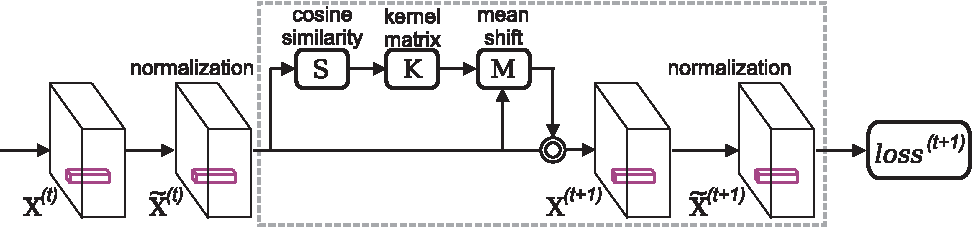
\includegraphics[width=1\linewidth]{meanShiftGroupingModule_only} % meanShiftGroupingModule_unrolled
   \vspace{-6mm}
   \caption{Recurrent mean shift grouping module is unrolled during training.
   %\TODO{(b) doesn't add much, maybe remove it? change G->K and P->M to be
   %consistent with changed notation below. It also seems skip arrow should go
   %from line representing X forward to M/P rather than from node S?}
   }
   \vspace{-3mm}
\label{fig:meanShiftGroupingModule}
\end{figure}

While we can directly train a model to predict embeddings as
described in the previous section, it is not clear how to generate the final
instance segmentation from the resulting (imperfect) embeddings. One can
utilize heuristic post-processing~\cite{de2017semantic} or utilize clustering
algorithms that estimate the number of instances~\cite{liang2015proposal},
but
these are not differentiable and thus unsatisfying. Instead, we introduce a
mean-shift grouping model (Fig.~\ref{fig:meanShiftGroupingModule})
which operates recurrently on the embedding space in order to congeal
the embedding vectors into a small number of instance labels.

Mean-shift and closely related algorithms~\cite{fukunaga1975estimation,
cheng1995mean, comaniciu1999mean, comaniciu2002mean} use kernel density
estimation to approximate the probability density from a set of samples and
then perform clustering on the input data by assigning or moving each sample to
the nearest mode (local maxima). From our perspective, the advantages of this
approach are (1) the final instance labels (modes) live in the same embedding
space as the initial data, (2) the recurrent dynamics of the clustering process
depend smoothing on the input allowing for easy backpropagation, (3) the
behavior depends on a single parameter, the kernel bandwidth, which is easily
interpretable and can be related to the margin used for the embedding loss.

\subsection{Mean Shift Clustering}
A common choice for non-parametric density estimation is to use the isotropic
multivariate normal kernel $K(\x, \x_i)= (2\pi)^{-D/2}\exp \Big(-
\frac{\delta^2}{2} \Vert\x - \x_i \Vert^2_2 \Big)$ and approximate the data
density non-parametrically as $p(x) = \frac{1}{N} \sum K(x,x_i)$. Since our
embedding vectors are unit norm, we instead use the von Mises-Fisher
distribution which is the natural extension of the multivariate normal to the
hypersphere~\cite{fisher1953dispersion,
banerjee2005clustering,mardia2009directional,kobayashi2010mises},
and is given by $K(\x,\x_i) \propto \exp( \delta \x^T \x_i )$.
The kernel bandwidth, $\delta$ determines the smoothness of the
kernel density estimate and is closely related to the margin used for learning
the embedding space. While it is straightforward to learn $\delta$ during
training, we instead set it to satisfy $\frac{1}{\delta}=\frac{1-\alpha}{3}$
throughout our experiments, such that the cluster separation (margin) in the
learned embedding space is three standard deviations.

We formulate the mean shift algorithm in a matrix form.  Let $\X \in
\RB^{D\times N}$ denote the stacked $N$ pixel embedding vectors of an image.
The kernel matrix is given by $\K = \exp(\delta \X^T\X) \in \RB^{N \times N}$.
Let $\D = \diag(\K^T\1)$ denote the diagonal matrix of total affinities,
referred to as the degree when $\K$ is viewed as a weighted graph
adjacency matrix. At each iteration, we compute the mean shift $\M =
\X\K\D^{-1} - \X$, which is the difference vector between $\X$ and the kernel
weighted average of $\X$. We then modify the embedding vectors by moving
them in the mean shift direction with step size $\eta$:
\begin{equation}
\begin{split}
\X \leftarrow & \X + \eta(\X\K\D^{-1} - \X)\\
\leftarrow & \X (\eta\K\D^{-1} + (1-\eta)\I)\\
\end{split}
\end{equation}
Note that unlike standard mean-shift mode finding, we recompute $\K$ at each
iteration.  These update dynamics are termed the explicit-$\eta$ method and
were analyzed by~\cite{carreira2008generalised}. When $\eta=1$ and the kernel
is Gaussian, this is also referred to as Gaussian Blurring Mean Shift (GBMS)
and has been shown to have cubic convergence~\cite{carreira2008generalised}
under appropriate conditions.  Unlike deep RNNs, the parameters of our
recurrent module are not learned and the forward dynamics are convergent under
general conditions.  In practice, we do not observe issues with exploding or
vanishing gradients during back-propagation through a finite number of
iterations~\footnote{Some intuition about stability may be gained by noting
that the eigenvalues of $\K\D^{-1}$ lie in the interval $[0,1]$, but we have
not been able to prove useful corresponding bounds on the spectrum of the
Jacobian.}.

Fig.~\ref{fig:mnist_demo} demonstrates a toy example of applying the method to
perform digit instance segmentation on synthetic images from
MNIST~\cite{lecun1998gradient}. We learn 3-dimensional embedding in order to
visualize the results before and after the mean shift grouping module.  From
the figure, we can see the mean shift grouping transforms the initial embedding
vectors to yield a small set of instance labels which are distinct (for negative
pairs) and compact (for positive pairs).

\begin{figure}[t]
\centering
   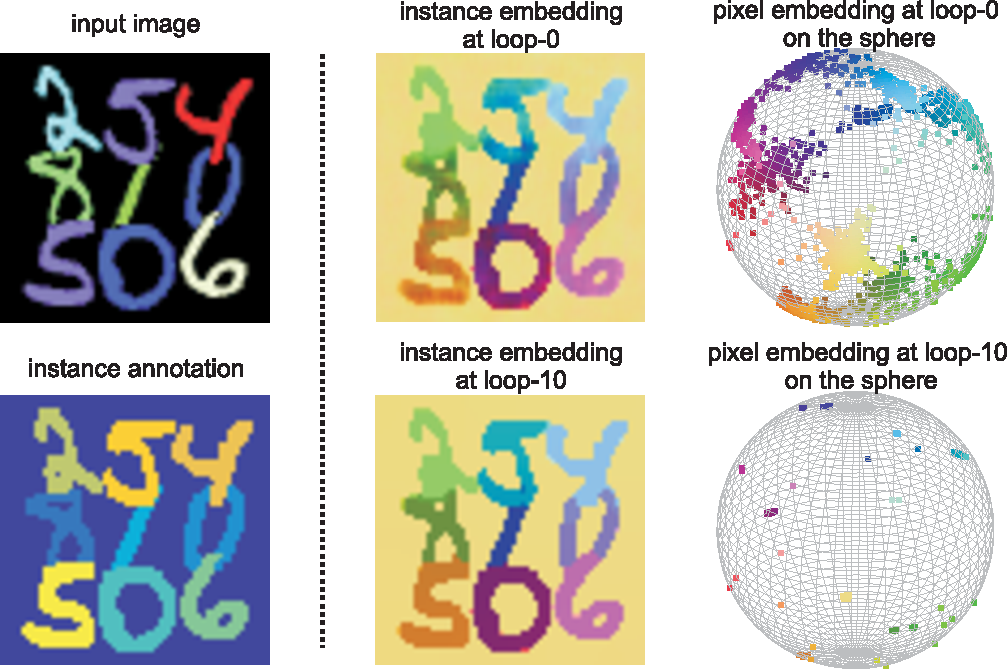
\includegraphics[width=0.95\linewidth]{mnist_demo}
   \vspace{-2mm}
   \caption{Demonstration of mean-shift grouping on a synthetic image and with
   ground-truth instance identities (left panel).  Right panel: the pixel
   embedding visualization at 3-dimensional embedding sphere (upper row) and
   after 10 iterations of recurrent mean-shift grouping (bottom row).
   }
   \vspace{-3mm}
\label{fig:mnist_demo}
\end{figure}


\subsection{End-to-end training}
It's straightforward to compute the derivatives of the recurrent mean shift
grouping module w.r.t $\X$ based on the the chain rule so our whole system is
end-to-end trainable through back-propagation.  Details about the derivative
computation can be found in the appendix.  To understand the benefit
of end-to-end training, we visualize the embedding gradient with and without
the grouping module (Fig.~\ref{fig:analysis_show_on_paper}).  Interestingly, we
observe that the gradient backpropagated through mean shift focuses on fixing
the embedding in uncertain regions, e.g.  instance boundaries, while suggesting
small magnitude updates for those errors which will be easily fixed by the
mean-shift iteration.

While we could simply apply the pairwise embedding loss to the final output of
the mean-shift grouping, in practice we accumulate the loss over all iterations
(including the initial embedding regression).
We unroll the recurrent grouping module into $T$ loops,
and accumulate the same loss function at the unrolled loop-$t$:
\begin{equation}
\small
\begin{split}
\ell^{t} =&  \sum_{k=1}^M  \sum_{i,j \in S_k} \frac{w^k_i w^k_j}{\vert S_k \vert}  \Big( \1_{\{y_i=y_j\}} ( 1 - s_{ij}^{t})   + \1_{\{y_i\not=y_j\}} [s^{t}_{ij}-\alpha]_{+} \Big) \\
\ell =& \sum_{t=1}^T \ell^{t}
\end{split}
\nonumber
\end{equation}
%\begin{eqnarray*}
%\small
%\ell^{t} &=&  \sum_{k=1}^M  \sum_{i,j \in S_k} \frac{w^k_i w^k_j}{\vert S_k \vert}  \Big( \1_{\{y_i=y_j\}} ( 1 - s_{ij}^{t})   + \1_{\{y_i\not=y_j\}} [s^{t}_{ij}-\alpha]_{+} \Big) \\
%\ell &=& \sum_{t=1}^T \ell^{t}
%\nonumber
%\end{eqnarray*}




\begin{figure}[t]
\centering
   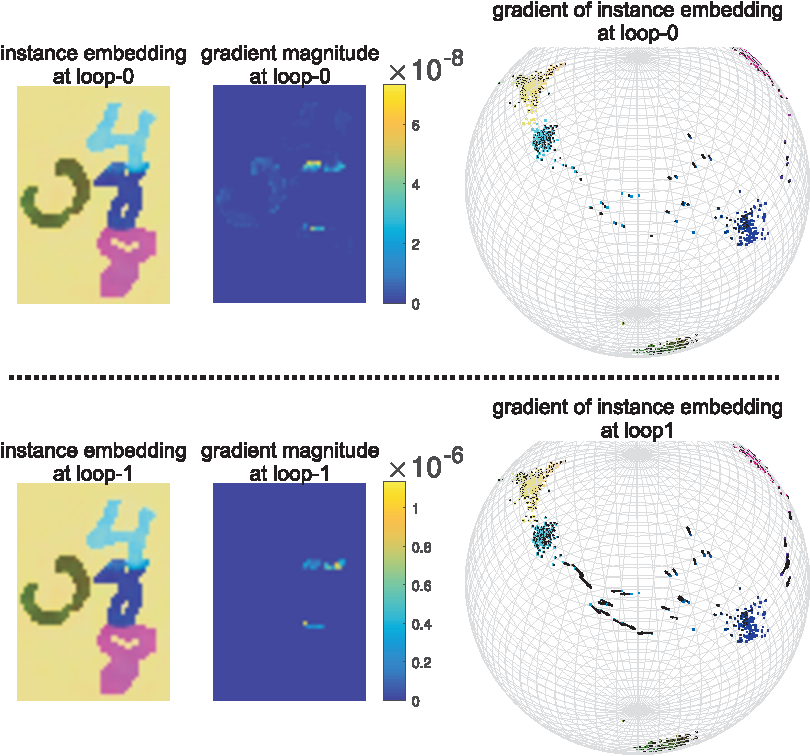
\includegraphics[width=1\linewidth]{analysis_show_on_paper_simple}
   \vspace{-6mm}
   \caption{To analyze the recurrent mean shift grouping module, we compare the
   embedding vector gradients with and without one loop of grouping.  The
   length of arrows in the projection demonstrates the gradient magnitude,
   which are also depicted in maps as the second column. Backpropagating the
   loss through the grouping module serves to focus updates on embeddings of
   ambiguous pixels near boundaries while ignoring pixels with small errors
   which will be corrected by the subsequent grouping process.
   }
   \vspace{-2mm}
\label{fig:analysis_show_on_paper}
\end{figure}

